\subsection{WP3 APAs (8 pages)}

{\bf Work package managers: J.\,Evans, A.\,Grant.}

\subsubsection{Introduction}

The APAs --- Anode Plane Assemblies --- are the most critical components of the TPC, collecting the ionisation charge, allowing reconstruction of detector activity with mm-scale resolution. These \SI{6x 2.3}{\metre} planes, one of which (built in the UK) is shown in Fig.~\ref{fig:CompleteAPA}, have four layers of \SI{150}{\micro\metre} beryllium-copper wire wound around them, as illustrated in Fig.~\ref{fig:APADiagram}. The layer structure is shown in Fig.~\ref{fig:APALayers}: from inside out, the layers are labelled $x$, $v$, $u$ and $g$. The $x$-layer and $g$-layer wires are aligned along the longest direction of the APA. The $v$-layer and $u$-layer wires are wound at an angle of \ang{35.7} to the the $x$-layer and $g$-layer. In between the inner $x$-layers, a grounding mesh is attached directly to the APA frame. A full description of the construction and functionality of the APAs can be found in Chapter 2 of Volume 2 of the DUNE Interim Design Report~\cite{ref:DUNEIDR}. Once installed in the DUNE Far Detectors, the APAs will hang vertically, in pairs one above another. The wires are read out by cold electronics at the top end of the top APA and the bottom end of the bottom APA.

\begin{figure}
\RawFloats
    \centering
    \begin{minipage}{.47\textwidth}
    \includegraphics[width=\linewidth]{figs/WP3/UKAPA.png}
    \captionof{figure}{A complete ProtoDUNE APA at the Daresbury Laboratory.}
    \label{fig:CompleteAPA}
    \end{minipage}%
\hspace{0.03\textwidth}
\begin{minipage}{.47\textwidth}
    \centering
    \includegraphics[width=\linewidth]{figs/WP3/WireWindingAngles.png}
    \captionof{figure}{The winding angles of the four wire layers.}
    \label{fig:APADiagram}
    \includegraphics[width=\linewidth]{figs/WP3/WireLayers.png}
    \captionof{figure}{The APA layer structure.}
    \label{fig:APALayers}
    \end{minipage}
\end{figure}

We propose to build 150 APAs in a factory at the Daresbury Laboratory. This will be half of the APAs required for the first two \SI{10}{\kilo\tonne} single-phase Far-Detector modules. The UK factory will be the biggest in the DUNE Collaboration; the remaining 150 APAs will be produced at two or three (to be defined) other factories in the US. By delivering this very significant part of the TPC instrumentation, the UK will have built its reputation as the most significant international partner in DUNE; we will also build up invaluable detector expertise that will allow UK physicists to be future Collaboration leaders.

The UK group that is proposing this project has demonstrated its ability to deliver by building two APAs for the ProtoDUNE detector and two for the SBND detector. The ProtoDUNE APA construction was led by Evans and Grant, who will be leading this WP. The key technical staff in this WP were also closely involved in the ProtoDUNE construction. The UK technical staff have been leading the development of the APA-production procedures, based on ProtoDUNE experience, to allow mass production for DUNE. In particular, Muir and Grant have redesigned the winding machine to speed up the wiring process.


\subsubsection{Work plan}

This project follows on from the UK pre-production project, as part of which we have updated the production procedure to allow mass production and are building the first of the four new winding machines that will make up the Daresbury factory. We are also preparing the area in the Daresbury Electron Hall that will house the factory.

WP3 begins at the start of the project, nominally on 1st October 2019. In the first nine months of the project, we will complete the build of the factory, assemble the remaining three winding machines and put in place all tooling and jigs. We will also define and document all quality-control procedures, ensure full documentation of the APA-production procedures, and set up all procurement contracts.

APA production will begin on 1st July 2020. As detailed below, the factory will produce one APA every ten working days, which are shipped to SURF in pairs. The APAs for the first \SI{10}{\kilo\tonne} module will be complete on 1st August 2023. Those for the second \SI{10}{\kilo\tonne} module will be complete on 30th June 2026.

To mitigate the risk that the second \SI{10}{\kilo\tonne} module will not use the single-phase technology, all procurement contracts will be placed in two batches. Contracts for the first module will be placed at the start of the project; contracts for the second module will be placed as soon as the technology decision is made (expected in 2021\todo{Is this the right date?}). Procurement of APA frames is the biggest procurement task; it will be ongoing throughout the project with two frames intended to be delivered, on average, every 15 working days. \todo{Is this right, Alan?} The remaining large procurement tasks (mesh panels and electronic components) will be complete by 2023, and the fully-tested components stored until needed.

\subsubsection{WP3.0 Management (J.\,Evans, A.\,Grant)}

%This WBS element runs for the entirety of the project.

\paragraph{WP3.0.1 Overall management} Managers: J.\,Evans, A.\,Grant.

Overall management for the work package will be provided by academic Evans (70\% FTE on the project) and project manager A.\,Grant (100\% FTE on the project). Evans and Grant oversaw the production of the UK protoDUNE APAs, and have been leading the UK pre-production project. 

Evans will focus on overall management, ensuring the UK groups are working together efficiently, that the correct people are hired into posts and that staff changeover is handled proactively. Evans will also be responsible for representing the Work Package to the international collaboration, primarily through the DUNE APA Consortium (led by Touramanis).

\paragraph{WP3.0.2 Quality management} Manager: Quality Manager

Strict quality-assurance procedures must be put in place from day one of the project. A dedicated Quality Manager, with previous experience of industry-standard quality assurance, will be employed to manage this aspect of the project. They will be responsible specifying and documenting the quality-control (QC) procedures at the start of the project, for ensuring the procedures are followed during production, and for documenting all QC data. The Quality Manager will work closely with the US groups that are building APAs to ensure that uniform procedures and requirements are defined across all APA factories.

Hiring of the Quality Manager will be one of the first high-priority tasks in the project.
The Quality Manager will be implicitly involved in all the WBS elements described below, and will be expected to be mobile: actively working with all the UK groups to assure quality in their areas of responsibility. The Quality Manager will be employed full time for the first three years of the project as the procedures are defined and the discipline of following the procedures instilled in the team. After this, the Quality Manager will drop to a 50\% FTE position, which will be adequate to allow continued oversight.

\paragraph{WP3.0.3 Procurement management}

Manager: A.\,Grant

The major procurement activities will make use of the professional procurement teams in place at the Universities: APA frames (Liverpool), Electrical components (Manchester), and mesh panels (Sheffield). All other equipment will be procured by the Daresbury Laboratory. High-level oversight for all procurement activities will be provided by A.\,Grant and overall project manager Preece. In the first year of the project, Gamez (deputy factory manager, and experienced member of the protoDUNE APA-production team) will focus a significant amount of time on supporting the procurement activities.\todo{we will need more substance on procurement, not sure if it is here or in the management section.}

Procurement is explicitly written into the work-package breakdown described below, with engineering and physicist effort assigned responsibility for the major procurement tasks. In the first nine months, the main focus of these staff will be on the tendering process, visiting potential suppliers to ensure they can achieve our requirements. Once production is underway, the team members will work closely with the suppliers, visiting on a weekly basis if necessary, to ensure QC procedures are followed and requirements are met.

As well as the major procurement tasks, a wide array of smaller mechanical parts are needed to produce an APA. This includes the beryllium-copper wire, the combs and comb-bases that maintain the wire spacing, epoxy, solder, and the APA protection panels that surround the APA before it goes into the shipping box. Overall responsibility for ensuring the supply of these components will fall with Gamez (supported by Manchester\_AP), who will be the deputy factory manager. Gamez was the lead PDRA for the protoDUNE APA production so is intimately acquainted with the required materials and therefore ideal to move into this core management position.
The first nine months of the project will see the search for suppliers who can provide materials at the rate required to keep the factory in stock. Once APA production is underway, WP3.4.3 details the responsibilities of the technical staff to monitor the level of materials at the factories. Any shortages will be reported to Gamez, and the responsibility lies in this WBS element to maintain the supply.

\paragraph{WP3.0.4 Communication with the international collaboration}

Manager: J.\,Evans.

Evans will represent the WP to the UK collaboration and the international DUNE collaboration. Within the UK project, Evans and A.\,Grant are part of the Project Management Committee, through which formal communication with the international collaboration will occur. They report directly to the project PI. Evans will coordinate WP activities with the international collaboration through the APA Consortium, ensuring regular reporting of UK activities. The APA consortium will also provide the mechanisms by which the UK team is informed about APA-production activities in the US. A close working relationship has already been built up between the UK and US teams that will continue into the construction phase. A particular focus of this WBS element will be the tracking and implementation of technical decisions taken by the wider collaboration, whether this be a small update to the APA design, or a major decision such as an FD module technology choice.

\subsubsection{WP3.1 APA mechanics (T.\,Jones, P.\,Sutcliffe)}
%This WBS element runs for the duration of the grant. It ends when all mechanical parts of all APAs are at Daresbury, fully tested and ready for installation onto an APA.

\paragraph{WP3.1.1 APA frames} Manager: P.\,Sutcliffe.

The APA frame is a \SI{6x2.3}{\metre} stainless steel structure (Fig.~\ref{fig:APAFrame}). The individual bars are selected from commercial section, end fittings welded on, and the whole frame screwed together on a jig that ensures flatness to the requirements listed in Tab.~\ref{tab:APAFlatness}. Compared to ProtoDUNE, the only change being made is that the width of the steel section is being increased to allow cables to be run along the insides of the frame sections. This will not require any changes to the APA production procedure.  To ensure that the frame supply is reliable, we will place contracts with two or three suppliers who will make frames in parallel. We expect to receive four frames every 30 working days. To aid in the frame QC, we will purchase a Total Station as part of the pre-production project, and budget for a replacement half way through the construction project.

\begin{figure}
\begin{floatrow}
\ffigbox{%
\centering
    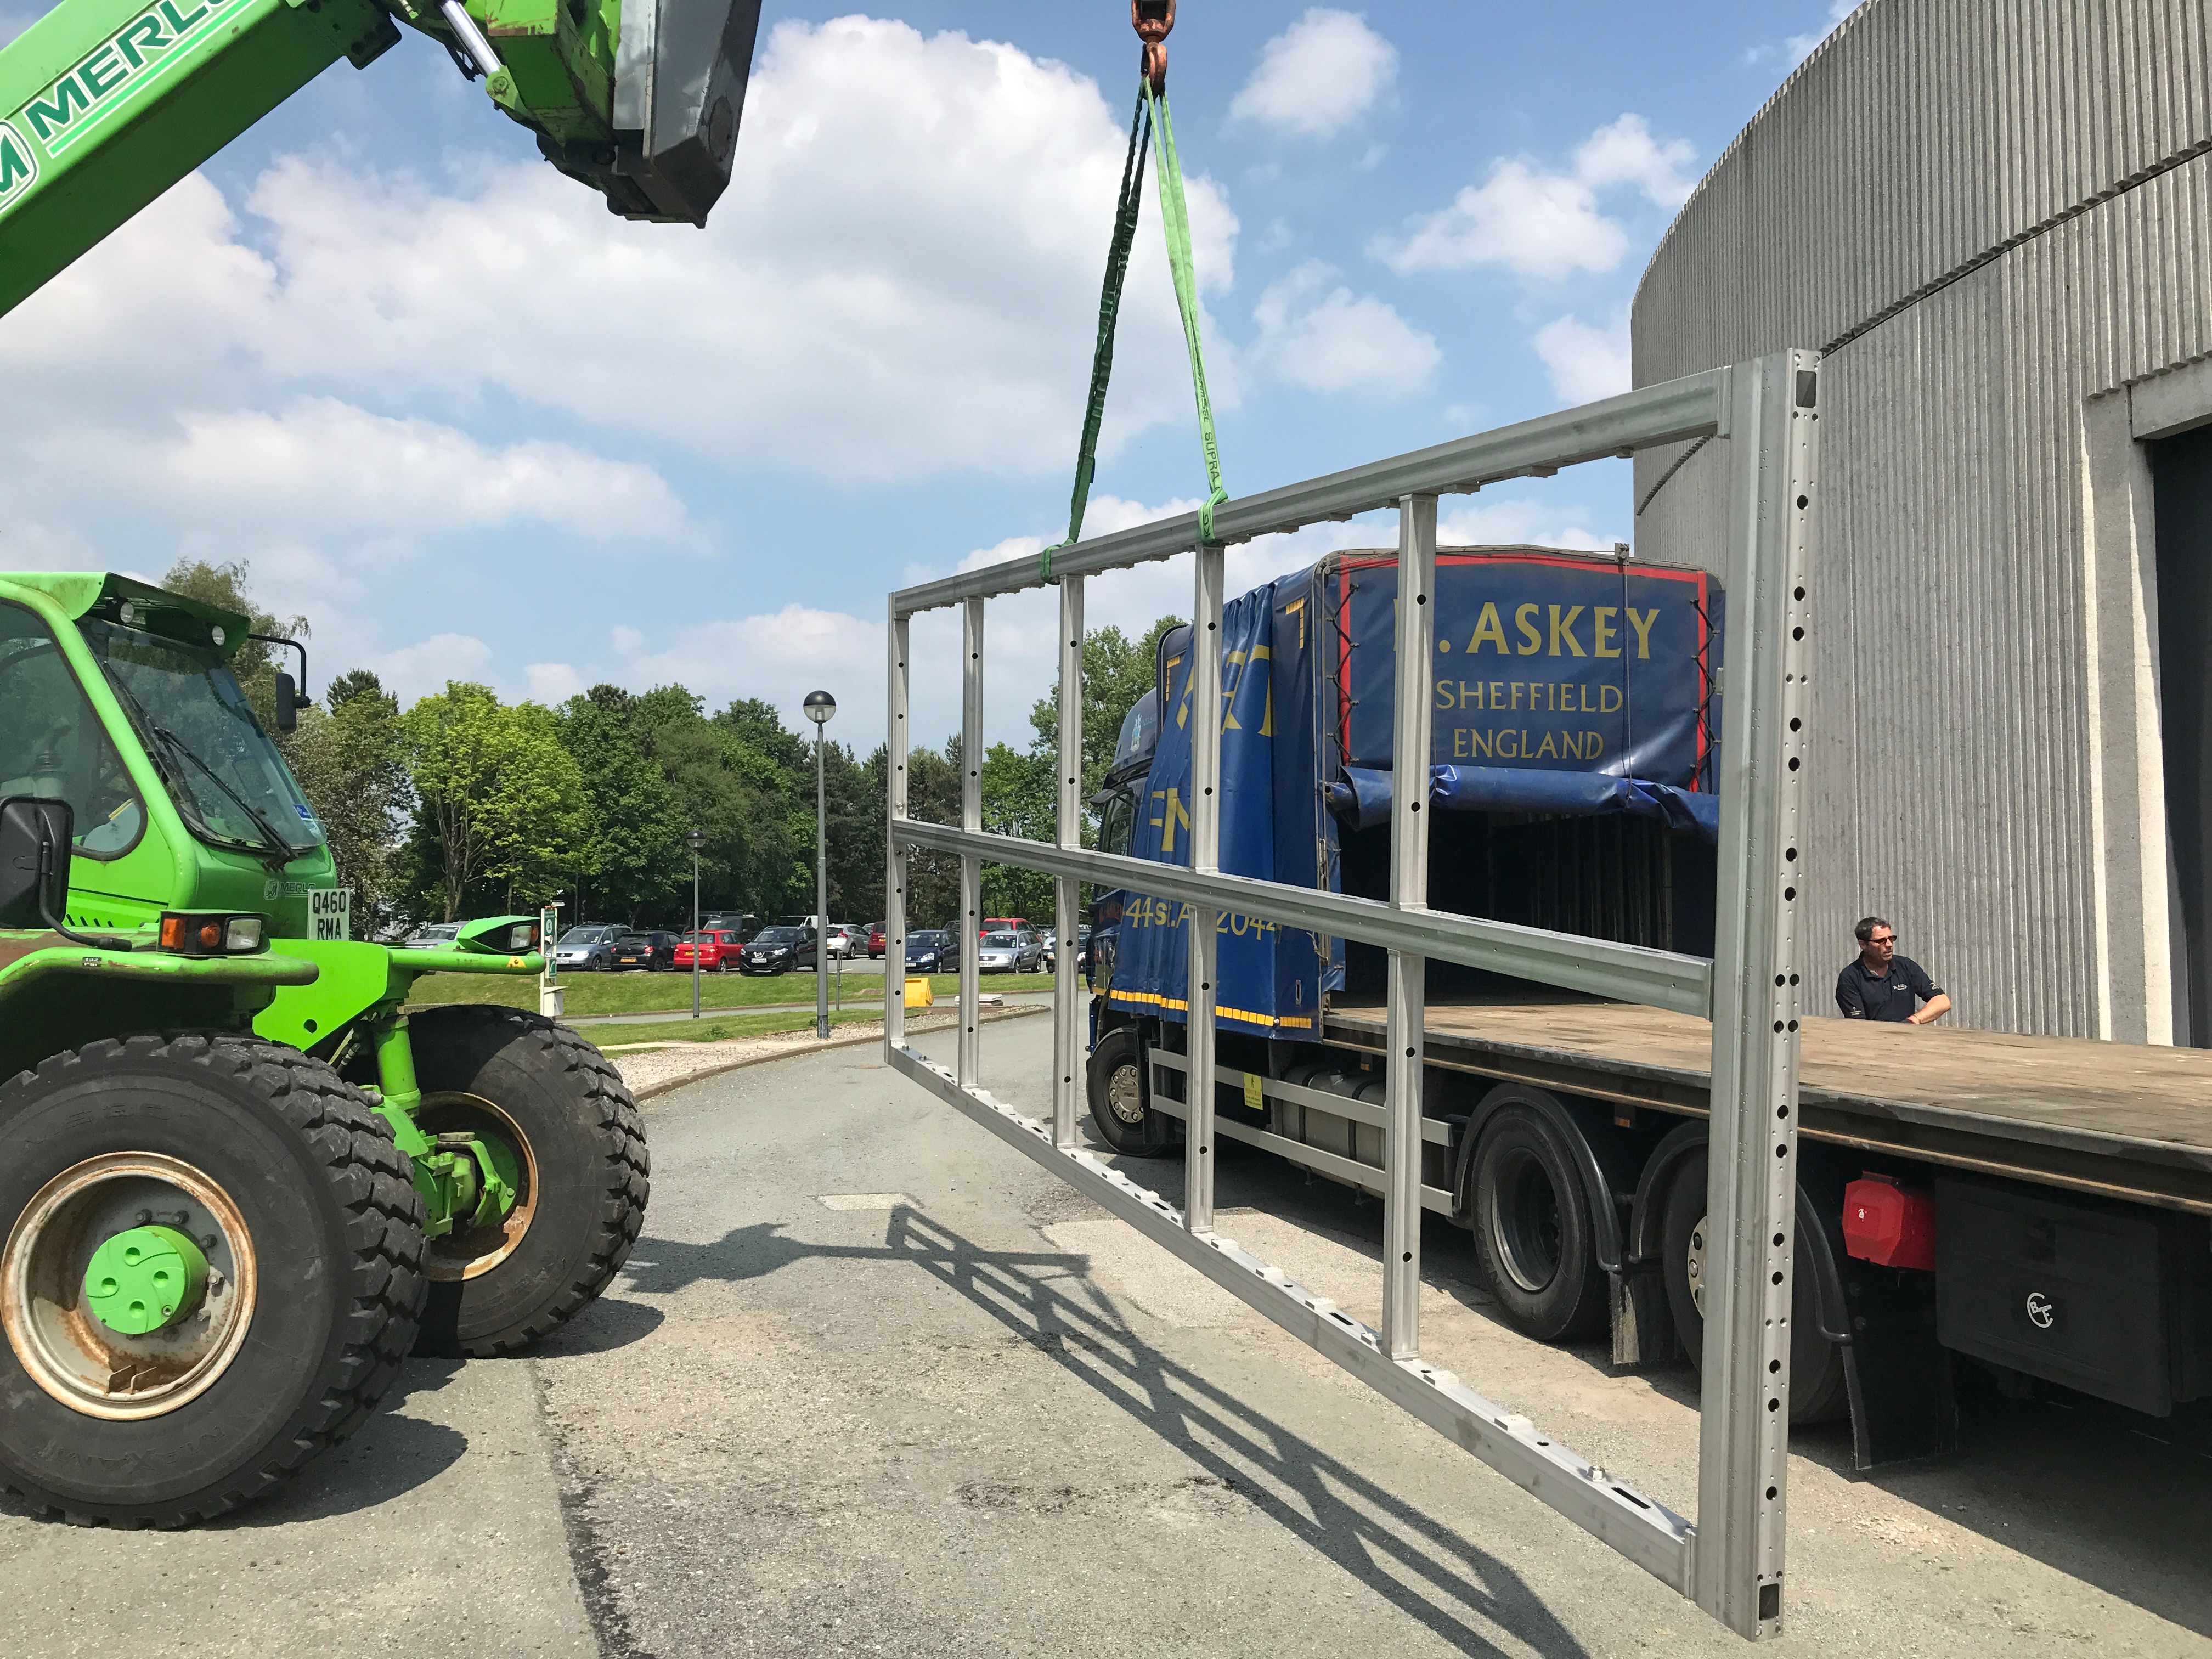
\includegraphics[width=0.37\textwidth]{figs/WP3/APAFrame.png}
}{%
    \caption{A protoDUNE APA frame.}
    \label{fig:APAFrame}
}
\capbtabbox{%
 \begin{tabular}{|l|c|}
\hline
    \multicolumn{1}{|c|}{\bf Criterion} & {\bf Tolerance} \\ \hline
    \multicolumn{2}{|c|}{\bf Flatness}\\
    Overall flatness & \SI{11}{\milli\metre} \\
    Overall bow & \SI{11}{\milli\metre}\\
    Overall twist & \SI{2}{\milli\metre / \metre}\\
    Twist in each zone of the frame & \SI{2}{\milli\metre / \metre}\\ \hline
    \multicolumn{2}{|c|}{\bf Fold --- front and back sides}\\
    Foot tube & \SI{1.2}{\milli\metre}\\
    Head tube & \SI{1.2}{\milli\metre}\\
    Ribs 1--4 & \SI{1.2}{\milli\metre}\\
    \hline
\end{tabular}
}{%
\caption{APA flatness requirements}
\label{tab:APAFlatness}
}
\end{floatrow}
\end{figure}

The engineers responsible for delivering the APA frames will be Peter Sutcliffe (supported by Liverpool\_Eng),  who currently leads the DUNE APA Consortium's testing, installation and integration working group, and Trevor Gamble, who oversaw the production of the ProtoDUNE frames. Additional oversight will be provided by T. Jones, who is highly experienced in managing large experimental construction projects such as the ATLAS Upgrade, and Payne who delivered the SBND CPA, supported by Liverpool\_AP. PDRA effort at Liverpool and Sheffield is assigned to perform analysis of QC data; technician effort is also assigned to support the work.


%In the first nine months of the project, close to 3.5 FTE is assigned to the setting up of the procurement contracts: visiting potential suppliers, defining QC procedures, and working with chosen suppliers to set up the procedures. Once the APA production is in full flow, this drops to around 3 FTE: every month, a team will spend five days on the premises of each of the suppliers, working with the supplier to perform QC on the frames. By working with the supplier like this, we maintain control of this most critical piece of QC; as a byproduct we also save money as the suppliers will not have to charge as much for the QC of the frames. To perform the frame QC, we will purchase a laser survey system such as a FARO Vantage, as part of the pre-production project. We budget £25k (plus VAT and contingency) to replace this system mid-way through the project to mitigate against its failure. This WBS element also includes oversight of shipping of completed frames to Daresbury, and dealing with any non-conformance found in the frames at Daresbury.

\paragraph{WP3.1.2 Mesh panels} Manager: T.\,Gamble.

A significant improvement on the protoDUNE APA production procedure is the use of UK-designed mesh panels that quickly and easily slot into the APA frames, reducing the production time of an APA by three days. We are currently fitting these mesh panels to the seventh protoDUNE APA (which will be used as an electronics test-stand) to ensure there are no unforeseen installation or operational issues.

The same technical team as is producing APA frames will be responsible for the mesh panels, with formal responsibility at Sheffield. The mesh panels will be procured and tested in the first four years of the grant, then stored until needed.

\paragraph{WP3.1.3 Wire} Manager: D.\,Gamez.

This is a capital-only WBS element that couples with the Gamez effort from WP3.0.3 to contain the procurement of the beryllium-copper wire.

\paragraph{WP3.1.4 Combs and comb bases} Manager: D.\,Gamez.

This is a capital-only WBS element that couples with the Gamez effort from WP3.0.3 to contain the procurement of the combs and comb bases.

\paragraph{WP3.1.5 Adhesive and fasteners} Manager: D.\,Gamez.

This is a capital-only WBS element that couples with the Gamez effort from WP3.0.3 to contain the procurement of the various epoxies, screws and other fasteners.

\subsubsection{WP3.2 Electrical components (J.\,Pater, M.\,Perry)}

%This WBS element runs for the first four years of the project. It ends when all electrical components are fully tested and in storage, ready for installation onto an APA.

\paragraph{WP3.2.1 PCB procurement}

Manager: J.\,Pater.

The project will require the procurement, testing and installation of more than 40,000 PCBs. The majority of the PCBs are the geometry boards onto which the APA wires are soldered; these consist of no components, only tracks. There are 204 geometry boards on each APA, of 25 different types. On each APA, there are also 20 CR boards, 20 $g$-bias filter boards and one SHV board, which contain components. The procurement of the boards, along with all testing, will be led by applied physicist Pater (an experienced manager of major ATLAS Upgrade work packages), and experienced electronics engineer Perry. All procurement and testing will completed in the first four years of the project.

\paragraph{WP3.2.2 PCB reception testing}

Manager: M.\,Perry.

After production, the geometry boards must be machined to allow the alignment teeth to be installed. The production company will send the boards straight to a machining company, who will then send the boards on to the testing sites.

The PCB testing will be divided between four sites (Cambridge, Lancaster, Manchester and Sheffield). The testing is a major logistical task due to the number of boards, and it is vital that the testing does not fall behind schedule and starve the factory of boards. Having multiple testing sites is therefore essential.

The geometry boards will be first tested for size, and then for continuity and isolation between adjacent tracks. The CR, $g$-bias filter and SHV boards will be tested to ensure functionality of all components. To simplify the logistics, each testing site will focus on a different type of board, but full written procedures will allow one site's tasks to be taken over by another site should a problem or delay occur. Cambridge and Sheffield will focus on geometry boards; Lancaster and Manchester will be responsible for boards with components and a smaller fraction of the geometry boards. Between the sites, we will be able to sets all the boards for a single APA in one day.

\paragraph{WP3.2.3 Board assembly}

Manager: M. Perry.

Board assembly will occur at the testing sites; for each APA's-worth of boards, this will happen in the two days after the testing.
Step one is the installation of the mill-max pins which allow the boards to connect together.
The teeth, which provide the alignment of the APA wires as they run off the geometry boards, must then be glued to the boards.  Alignment of the teeth is provided by jigs; a different jig is needed for each board type, and the testing sites will have enough jigs to allow, between the sites, all the boards for one APA to have the teeth attached in parallel. Once the teeth are attached, the epoxy must dry overnight. The following day, the boards for one APA are packaged up and shipped to the factory.

\paragraph{WP3.2.4 Wire harnesses}

Each APA requires one wire harness, which forms the connection to the cold electronics. These harnesses will be assembled at the board testing sites.

\subsubsection{WP3.3 Factory setup (A.\,Grant)}

%This WBS element runs for the first nine months of the project. It ends when the factory setup is complete, and all four production lines have begun operations.

\paragraph{WP3.3.1 Factory infrastructure} Manager: A.\,Grant.

The APA factory, shown in Fig.~\ref{fig:APAFactory}, will be in the Electron Hall Inner Hall at the Daresbury Laboratory. Work is already underway to prepare the area, repairing the floor, and installing new cranes and all infrastructure needed such as power and the clean tent. A.\,Grant will oversee this WBS element, and the factory area will be ready for installation of winding machines in advance of October 2019. The current schedule is for work the Inner Hall work to be complete by February 2019, and the plant room (shipping area) to be complete by April 2019. This WBS element also covers the purchasing of the access tooling needed for production (ladders, working platforms), the installation of storage racks, and the setting up of materials-preparation tables.

\begin{figure}
\RawFloats
    \centering
\begin{minipage}{.47\textwidth}
  \centering
    \includegraphics[width=\linewidth]{figs/WP3/FactoryLayout.png}
    \captionof{figure}{The APA factory at Daresbury.}
    \label{fig:APAFactory}
    \end{minipage}
\hspace{0.03\textwidth}
\begin{minipage}{.47\textwidth}
    \centering
    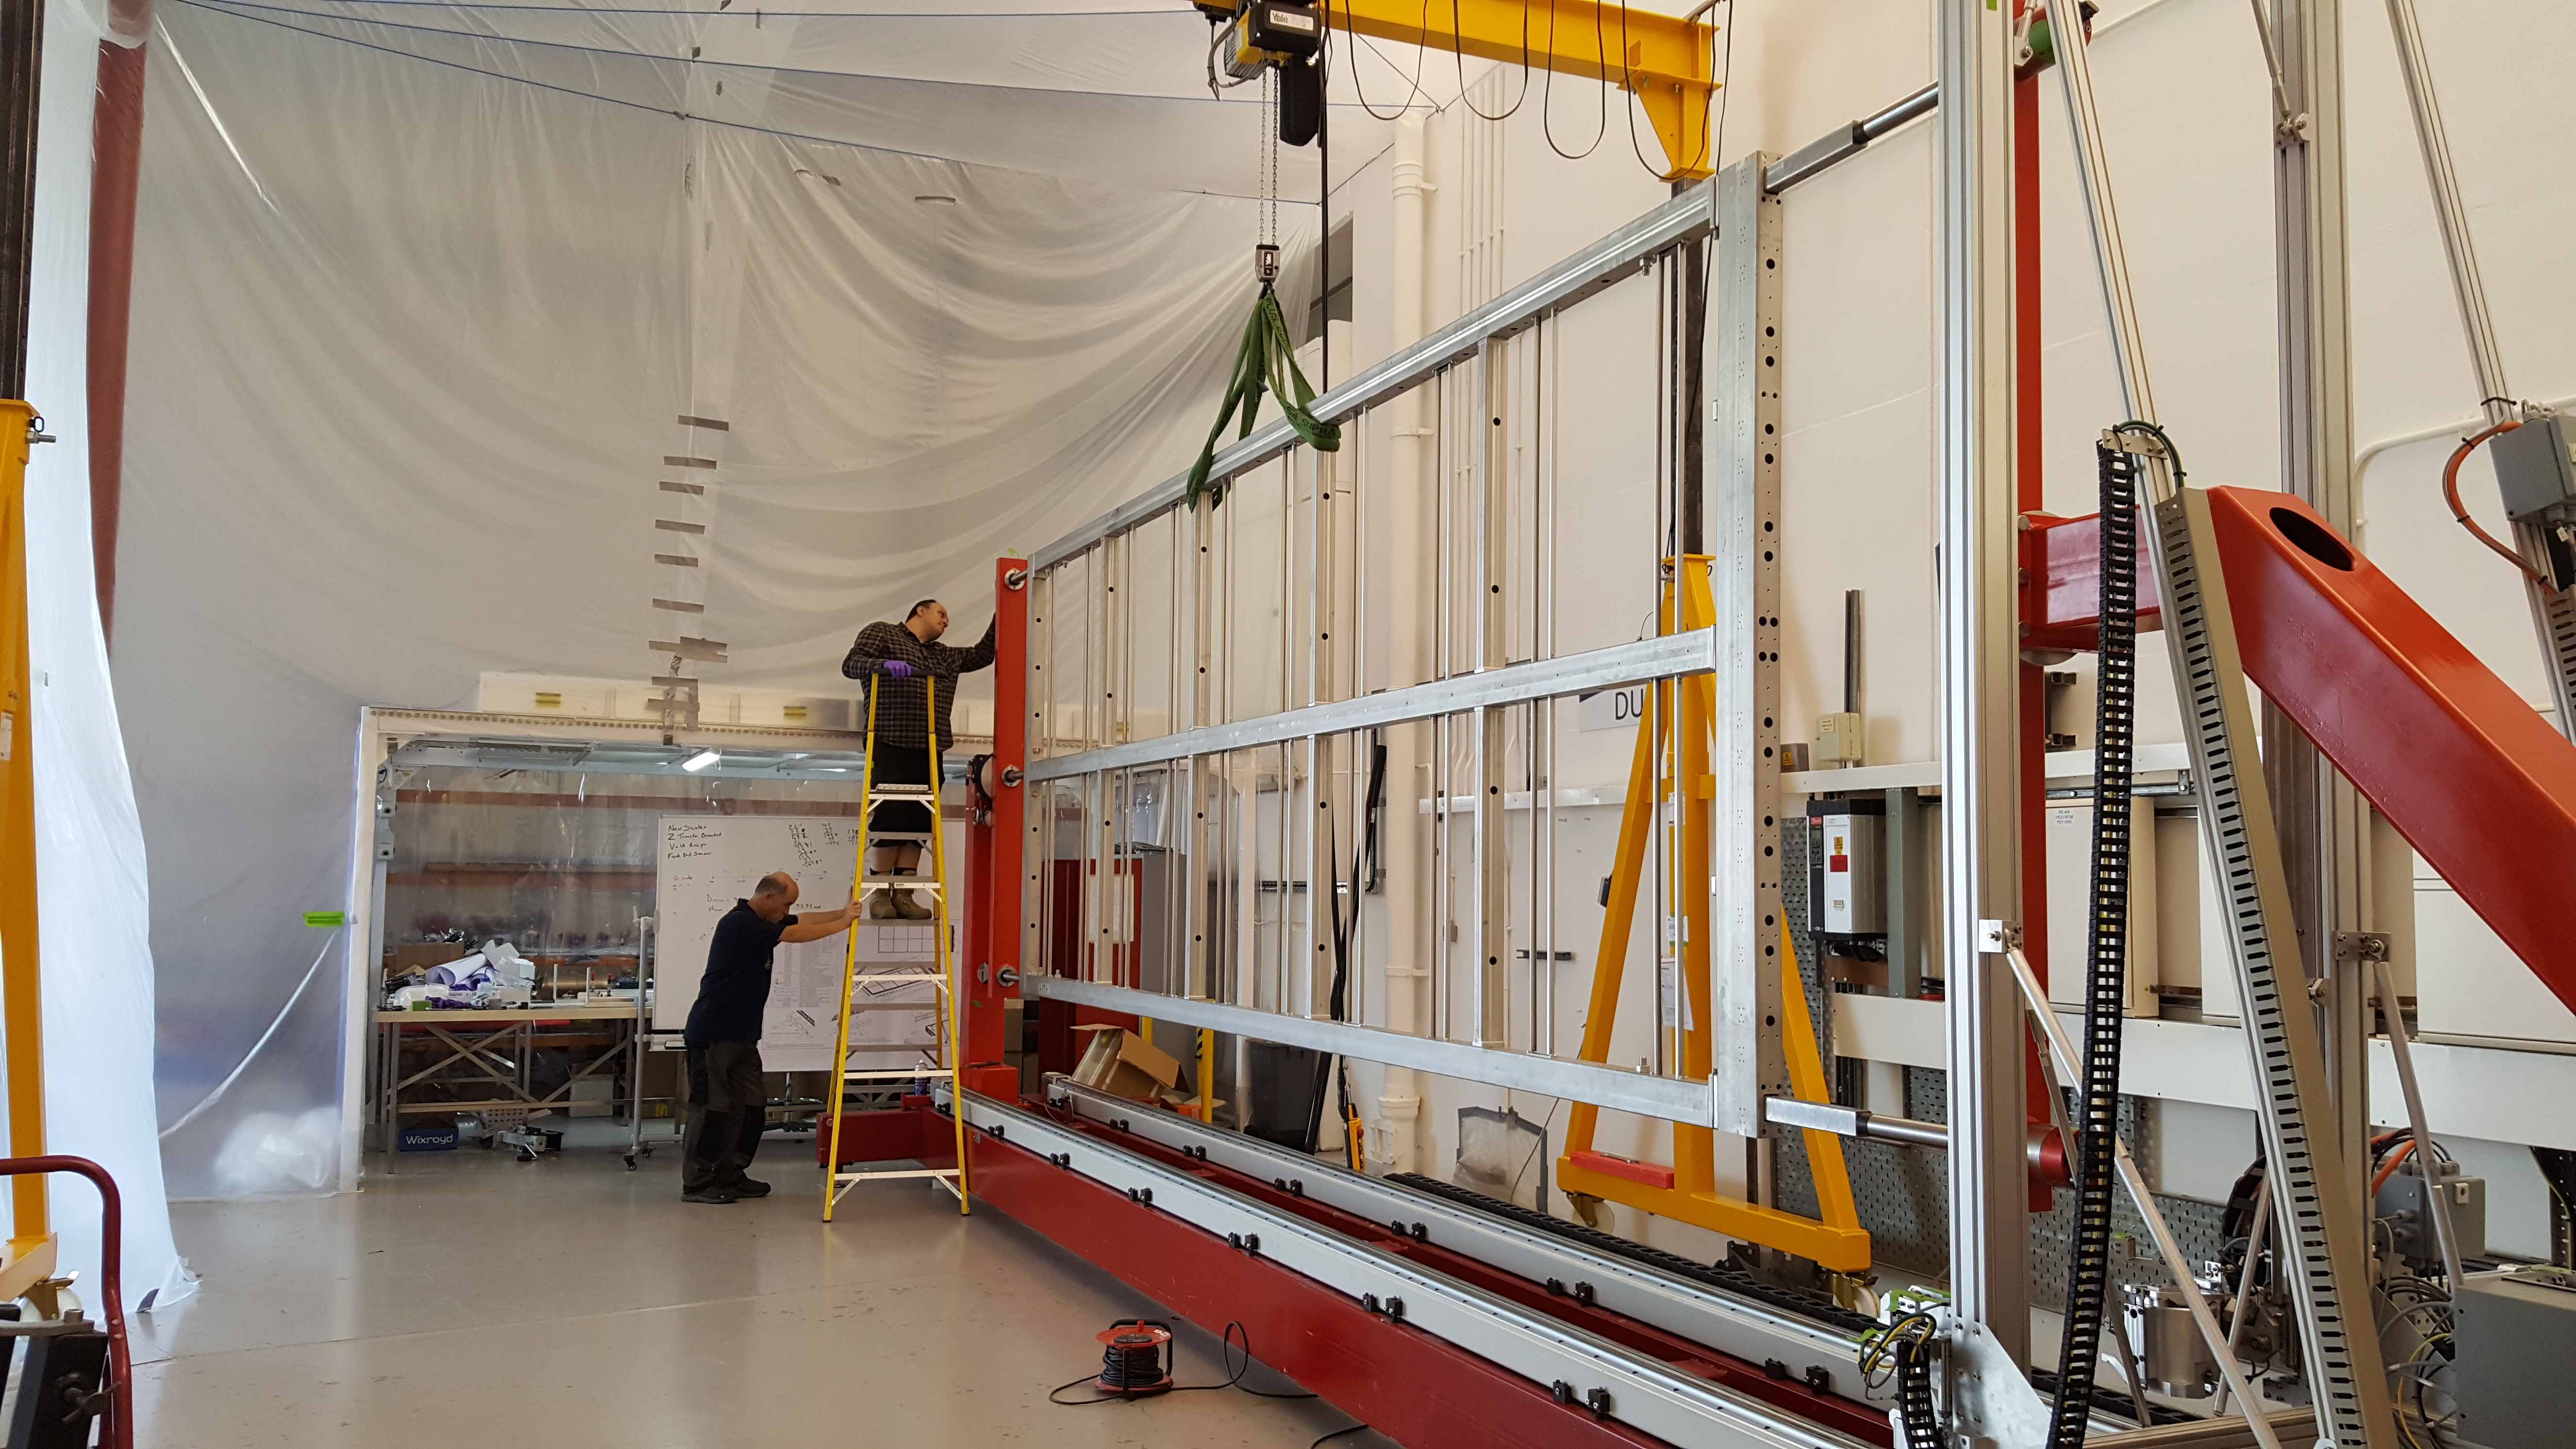
\includegraphics[width=\linewidth]{figs/WP3/TheNewWinder.png}
    \captionof{figure}{The APA-winding machine}
    \label{fig:WindingMachine}
\end{minipage}
\end{figure}

\paragraph{WP3.3.2 Winding machines} Manager: A.\,Muir.

This is a capital-only WBS element that couples with effort from WP3.3.5 to contain the procurement of the parts for the three remaining winding machines.

\paragraph{WP3.3.3 Winding heads} Manager: A.\,Muir.

This is a capital-only WBS element that couples with effort from WP3.3.5 to contain the procurement of the winding heads for the three remaining winding machines.

\paragraph{WP3.3.4 Process carts} Manager: A.\,Muir.

This is a capital-only WBS element that couples with effort from WP3.3.6 to contain the procurement of the parts for the eight remaining process carts.

\paragraph{WP3.3.5 Factory build --- winding machines} Manager: A.\,Muir.

The DUNE winding machine was originally designed by engineers at PSL (Madison, Wisconsin), and has been improved upon by UK engineers, led by Muir, to allow a much faster winding process with significantly less handling of the APA, and improved wire-tension control. The first of the new winding machines has, as of September 2018, been built at Daresbury (Fig.~\ref{fig:WindingMachine}) and is now being commissioned. This will be the first of the four factory winding machines. Through the remainder of 2018, it will be used to wire a seventh ProtoDUNE-style APA, which will be used as an electronics test stand. This winding exercise will allow us to run through all the new production processes and to iron out any problems with the new machine.

This WBS element will see Muir oversee the build of the three remaining machines in the first nine months of the project, and the move of the existing machine down from the Daresbury Tower area to the factory area.

\paragraph{WP3.3.6 Glue jigs, tooling, process carts and ancillary equipment} Manager: A.\,Muir.

Before and after winding, the APAs are handled on process carts. As well as allowing the APAs to be moved around the factory, these process carts are where photon-detector rails and mesh panels are installed, and where cover boards and APA protection panels are installed. We currently have two process carts, and will purchase a further 8. This will give us two process carts per winding machine, and two additional carts to allow complete APAs to be moved around the factory and taken to the shipping area.

This WBS element includes the purchase and construction of all the jigs required for APA construction, such as comb-assembly and comb-installation jigs, and jigs for applying epoxy to the geometry boards.

\subsubsection{WP3.4 Factory operations (D.\,Gamez, A.\,Grant)}
%This WBS element begins in month 10 of the project, and runs to the project end. It begins when construction of the first APA starts in the factory; it ends when the final APA is shipped out of the factory.

\paragraph{WP3.4.1 Factory management} Managers: D.\,Gamez, A.\,Grant.

A.\,Grant will take the role of Factory Manager, and D.\,Gamez that of Deputy Factory Manager. Between them, they will provide full-time oversight of factory operations. They are both highly experienced in APA production from the UK protoDUNE activities.

\paragraph{WP3.4.2 Factory maintenance} Manager: A. Muir.

Maintaining the functionality of all four winding machines and their associated production lines, plus the factory infrastructure, is vital to maintaining the project schedule. Around 2 FTE is dedicated to factory maintenance throughout the project, a mixture of technician, engineer and PDRA effort. Technician effort will focus on the maintenance and replacement of the various jigs. At Daresbury, specialist electronics, mechanical and controls engineer time is dedicated to maintaining the winding machine. The first ports of call for winder software problems will be the specialist winding technicians, and Manchester\_PDRA who will be an expert in the winder controls software. Effort from university engineering staff is also ring-fenced to be called on for factory maintenance: in case of a serious problem with a winder, an all-hands-on-deck attitude will be taken to get the factory running again as quickly as possible.

\paragraph{WP3.4.3 Materials management} Manager: D.\,Gamez.

It is vital that the factory not be starved of materials. Gamez (the deputy factory manager) will be responsible for overseeing the management of all materials supply. 50\% of one of the factory technicians will be dedicated to stock-keeping. When orders of new materials are required, this WBS element will feed into the relevant parts of WP3.1 and WP3.2 where procurement and supply of parts will be performed. 

\paragraph{WP3.4.4 APA production} Manager: A.\,Grant.

APA production is the central WBS element of the project. The factory consists of four production lines. Each production line is one winding machine and two process carts. The schedule for building a single APA is shown in Fig.~\ref{fig:FactorySchedule}, in terms of eight-hour shifts. It is assumed that the factory will run a single eight-hour shift with all four production lines in use on all standard working days. This then allows weekends and double-shifting to be used to regain any lost schedule. This schedule has been determined, in collaboration with US experts and the whole APA Consortium, based on ProtoDUNE experience and including known improvements the production process. The schedule is designed to be conservative, so as to include time for problem-solving and for factory maintenance, such that we have confidence that the project can stay on schedule from day one.


%\todo{We need a bit more information so that the reviewers get a fuzzy feeling that we are on top of these estimates. Say how this was determined, which saving have been assumed and how much time/effort contingency has been added.}

\begin{figure}
    \centering
    \includegraphics[angle=90,origin=c,width=\textwidth]{figs/WP3/FactorySchedule.png}
    \caption{The schedule for producing a single APA.}
    \label{fig:FactorySchedule}
\end{figure}

Although a single APA requires 50 shifts to be built, the schedule driver is the 40 shifts that the APA spends on the winder. We therefore aim to keep the winders in use at all time. Prior to winding, pre-production activities take place on a process cart; post-production take place on a second production cart. By having two production carts paired with each winding machine, this means that whilst the $n$th APA is on the winding machine, pre-production on the $(n+1)$th APA and post-production on the $(n-1)$th APA can be taking place. Thus the factory can produce four APAs every 40 working days.

The core technician team consists of 13.5 technicians who will be based full-time at the Daresbury factory. Seven of the technicians, along with the 50\% technician, are assigned entirely to APA production, and will be the expert winder operators. The other six full-time technicians are assigned 50\% to APA production, focusing on the pre-winding and post-winding activities on the process carts. The other 50\% of the time of these six technicians are assigned to QC documentation, factory maintenance, materials management and shipping.

%Daresbury: 3.5, 1.5 is just winding. 2x0.5 is production, with maintenance and materials.
%Lancaster: 2 techs, both 50\% QC
%Liverpool: 2 techs, both 100\% production
%Manchester 3 techs: 1 is 100\% production, the other two shipping and maintenance
%Sheffield: 3 techs, 100\% production

In addition to the core technician team, fractions of university technical staff and PDRAs are earmarked for APA production so that we can call on them to cover holidays and sickness of members of the core team. We will also make use of PhD students as necessary to maintain the schedule.

\paragraph{WP3.4.5 APA quality control and documentation} Manager: Quality Manager.

The QC procedures will have been defined in WP3.0.2. This WBS element is where the APA production team follows the QC procedures, takes any remedial action, documents the results and produces non-conformance documents as required. The documentation will take the form of travellers that stay with the APAs. For ProtoDUNE, paper travellers were used. For DUNE, the Quality Manager will oversee the development of online, iPad-based travellers that will allow easier storage of QC data in databases, and which can be rolled out to the US factories.

\subsubsection{WP3.5 APA shipping (D.\,Gamez, T.\,Jones)}
%This WBS element runs through the entirety of the project, ending when the last UK APA has been delivered to SURF and signed off as ready for installation.

\paragraph{WP3.5.1 Shipping boxes} Manager: J.\,Freestone.

An APA transport frame holds two complete APAs and fits inside a standard shipping container. Engineers from Manchester and Liverpool will work together at the start of the project to find suppliers that can provide the transport frames at the required rate. Technical effort has been assigned at the universities for final assembly of the transport frames.


\paragraph{WP3.5.2 Shipping management} Manager: D.\,Gamez.

Transport of completed APAs will be by ship across the Atlantic, then by road to SURF. Transport can begin as soon as the Integration and Test Facility (ITF) is available at SURF, currently scheduled for April 2021. Before this time, completed APAs will be stored in commercial storage in the UK. Once shipping begins, APAs will be shipped out of the factory as soon as a pair of APAs is ready to fill a shipping container.

The APAs will be instrumented with vibration monitors. PDRA effort is assigned to analyse the data from these monitors. Any findings from these, or findings of damage at the ITF, will be fed back to the engineers responsible for the shipping boxes (WP3.5.1) who will make any necessary changes to the design.

\subsubsection{WP3.6 Integration (N.\,McConkey, P.\,Sutcliffe)}
%This WBS element runs for the full period of the project, and ends when the final UK APA is installed into the DUNE Far Detector.

\paragraph{WP3.6.1 Contributions to technical coordination} Manager: A. Muir.

Engineer effort dedicated to working as part of the international collaboration's technical coordination team can be reclaimed against the Common Fund requirement as a contribution in kind. 80\% of Muir, once the factory has been set up, is assigned to working for the collaboration's Technical Coordinator.

\paragraph{WP3.6.2 Detector studies} Managers: C.\,Griffith, N.\,McConkey.

As production progresses, questions will arise about the APA design. There will also be non-conformances in APAs, and studies will be needed to understand whether the non-conformances can be accepted, or whether it will have to be rectified. PDRA effort is assigned to performing these studies.

\paragraph{WP3.6.3 APA reception testing at SURF} Manager: N.\,McConkey.

It is vital that UK physicists, in particular PDRAs, have a presence at SURF during construction, both to engage the UK in the installation and to build the reputation of our PDRAs within the international collaboration. Each PDRA requested in this WP will spend one year on LTA at SURF working with the integration teams there, focusing on APA reception testing.

\subsubsection{Deliverables and Milestones}

\todo{Alan and Roy: can you write this?}

\subsubsection{Business Case}

This WP will engage a significant amount of UK business, in particular the production APA frames, PCBs, mesh panels and shipping boxes. We will be working in those companies, building their capability in the data-analysis involved in quality assurance.\todo{this needs to be extended. Use information from Benefit Realisation WS.}